\chapter{Foundations of artificial intelligence and machine learning paradigms}
\label{sec:foundations_and_paradigms}

\section{Course architecture and the 3-tier examination framework}
\label{sec:academic_environment}

The graduate curriculum in \emph{Advanced Machine Learning} at Politecnico di Torino (Course Codes: \texttt{01URWOV} / \texttt{01URWYG}, 6 CFU) is structured to transition students from passive consumers of machine learning APIs into rigorous theoretical researchers and deep learning engineers. The curriculum operates under the academic direction of the DAUIN, VANDAL Lab, and ELLIS Unit Turin teams.

\begin{figure}[htbp]
\centering
\resizebox{0.96\linewidth}{!}{
\begin{tikzpicture}[
  tier/.style={rectangle, rounded corners=2.5mm, draw=politoNavy, fill=skyBlue!12, thick, text width=4.6cm, minimum height=3.4cm, inner sep=3mm, align=left},
  dimlabel/.style={font=\bfseries\sffamily, text=politoNavy}
]
\node[tier] (T1) at (0, 0) {
  \textbf{\color{politoNavy}Tier 1: Research Paper}\par
  \textbf{\color{examred}Weight: 6--10 Points}\par\vspace{1ex}
  \footnotesize
  $\bullet$ 12-minute strict group presentation\par
  $\bullet$ Teams of exactly 4 students\par
  $\bullet$ Seminal papers (CVPR, NeurIPS, ICLR)\par
  $\bullet$ Mathematical loss deconstruction
};
\node[tier, right=0.6cm of T1] (T2) {
  \textbf{\color{politoNavy}Tier 2: Mentored Project}\par
  \textbf{\color{examred}Weight: 6--10 Points}\par\vspace{1ex}
  \footnotesize
  $\bullet$ Applied experimental challenge\par
  $\bullet$ Continuous VANDAL Lab mentorship\par
  $\bullet$ Comprehensive technical PDF report\par
  $\bullet$ Submission 10 days before oral exam
};
\node[tier, right=0.6cm of T2] (T3) {
  \textbf{\color{politoNavy}Tier 3: Theoretical Oral}\par
  \textbf{\color{examred}Weight: 6--10 Points}\par\vspace{1ex}
  \footnotesize
  $\bullet$ Individual comprehensive defense\par
  $\bullet$ Project methodology questioning\par
  $\bullet$ First-principles derivations across all syllabus modules\par
  $\bullet$ Required for top honors (30L)
};
\node[rectangle, rounded corners=2mm, draw=politoNavy, fill=politoNavy, text=white, font=\bfseries\sffamily, text width=8.5cm, align=center, below=0.6cm of T2] (Total) {
  Final Evaluation: Sum of Three Tiers (18--30L Points)
};
\draw[-{Stealth[scale=1.1]}, thick, draw=politoNavy] (T1.south) -- ++(0,-0.3) -| (Total.160);
\draw[-{Stealth[scale=1.1]}, thick, draw=politoNavy] (T2.south) -- (Total.north);
\draw[-{Stealth[scale=1.1]}, thick, draw=politoNavy] (T3.south) -- ++(0,-0.3) -| (Total.20);
\end{tikzpicture}
}
\caption{The 3-tier examination and evaluation architecture of the Advanced Machine Learning course at Politecnico di Torino. The final grade combines three complementary assessments: a 12-minute group research paper presentation (6--10 points), a mentored experimental lab project (6--10 points), and a rigorous theoretical oral examination (6--10 points).}
\label{fig:slide_exam_framework}
\end{figure}

\subsection{The 3-tier evaluation architecture}
\label{sec:exam_evaluation_tiers}

As formalized in Figure~\ref{fig:slide_exam_framework}, successful completion of the course requires mastering three complementary evaluation tiers:
\begin{enumerate}
  \item \textbf{Seminal Research Paper Presentation (6--10 Points)}:
    \begin{itemize}[noitemsep]
      \item Teams of exactly 4 students deliver a strictly timed 12-minute presentation breaking down a seminal research paper published within the last 3--7 years in top computer vision and machine learning venues (CVPR, ICCV, ECCV, NeurIPS, ICLR, ICML, TPAMI).
      \item Evaluation criteria focus on problem formulation, architectural mechanisms, mathematical loss deconstructions, ablation analysis, and unstated assumptions.
    \end{itemize}
  \item \textbf{Mentored Group Project (6--10 Points)}:
    \begin{itemize}[noitemsep]
      \item Student teams tackle applied research challenges under the continuous mentorship of VANDAL Lab teaching assistants.
      \item Teams submit a comprehensive technical experimental report in PDF format strictly 10 days prior to the examination date.
    \end{itemize}
  \item \textbf{Theoretical Oral Examination (6--10 Points)}:
    \begin{itemize}[noitemsep]
      \item A comprehensive individual defense covering both the experimental project and \textbf{mandatory theoretical questioning spanning all course syllabus modules}.
      \item To achieve top honors ($30\text{L}$), students must articulate first-principles derivations, declare explicit tensor dimensions, state foundational statistical assumptions, and navigate loss landscape geometries. Hand-waving or purely qualitative answers are insufficient.
    \end{itemize}
\end{enumerate}

---

\section{What is artificial intelligence? From logicism to computational rationality}
\label{sec:what_is_ai}

To understand modern machine learning, one must first deconstruct the historical evolution and foundational definitions of artificial intelligence. In their seminal treatise, Russell and Norvig~\cite{russell2020artificial} observe that artificial intelligence has historically been defined along two primary orthogonal axes:
\begin{enumerate}
  \item \textbf{Thinking vs. Acting}: Does intelligence concern internal cognitive and inferential processes (how an agent reasons, plans, and structures beliefs), or does it concern external, observable behavior and agency (how an agent acts in and interacts with its environment)?
  \item \textbf{Human-Centric vs. Rationality-Centric}: Is the benchmark of success measured by fidelity to human performance (including human biological idiosyncrasies, memory limitations, and psychological cognitive biases), or is it measured by adherence to an idealized, normative standard of rationality (doing the mathematically ``right thing'')?
\end{enumerate}

These two orthogonal dimensions define a $2 \times 2$ taxonomy spanning four distinct historical paradigms of artificial intelligence, formalized structurally in Figure~\ref{fig:ai_quadrants_schema}.

\begin{figure}[htbp]
\centering
\resizebox{0.96\linewidth}{!}{
\begin{tikzpicture}[
  box/.style={rectangle, rounded corners=2.5mm, draw=politoNavy, fill=skyBlue!12, thick, text width=7.0cm, minimum height=3.5cm, inner sep=3.5mm},
  dimlabel/.style={font=\bfseries\sffamily, text=politoNavy!90!black, align=center}
]
\node[box] (TH) at (0, 0) {
  \textbf{\color{politoNavy}1. Thinking Humanly}\par\vspace{1ex}
  \footnotesize
  $\bullet$ Cognitive science modeling of inner human thought\par
  $\bullet$ Methodologies: Introspection, psychological testing, fMRI\par
  $\bullet$ Newell \& Simon's General Problem Solver (GPS, 1961)\par
  $\bullet$ Compares reasoning sequences and timing against human trials\par
  $\bullet$ \textit{Evaluation Metric}: Empirical fidelity to human cognition
};
\node[box, right=1.0cm of TH] (TR) {
  \textbf{\color{politoNavy}2. Thinking Rationally}\par\vspace{1ex}
  \footnotesize
  $\bullet$ The ``Laws of Thought'' formal logicist tradition\par
  $\bullet$ Aristotle's syllogisms and deductive inference rules\par
  $\bullet$ First-Order Logic (FOL) \& automated theorem proving\par
  $\bullet$ Robinson's resolution refutation algorithm (1965)\par
  $\bullet$ \textit{Evaluation Metric}: Mathematical deductive soundness
};
\node[box, below=1.0cm of TH] (AH) {
  \textbf{\color{politoNavy}3. Acting Humanly}\par\vspace{1ex}
  \footnotesize
  $\bullet$ Alan Turing's Imitation Game (1950)\par
  $\bullet$ Behavioral operational test bypassing metaphysics\par
  $\bullet$ Core components: NLP, KR, Automated Reasoning, ML\par
  $\bullet$ Total Turing Test: Computer Vision + Physical Robotics\par
  $\bullet$ \textit{Evaluation Metric}: Indistinguishability from human responses
};
\node[box, right=1.0cm of AH] (AR) {
  \textbf{\color{politoNavy}4. Acting Rationally}\par\vspace{1ex}
  \footnotesize
  $\bullet$ The Rational Agent paradigm (Modern AI Standard Model)\par
  $\bullet$ Autonomous entities executing actions to maximize expected utility\par
  $\bullet$ Mathematical formulation: $a^* = \arg\max_a \mathbb{E}[U \mid \text{percepts}]$\par
  $\bullet$ Unifies AI, control theory, operations research, and economics\par
  $\bullet$ \textit{Evaluation Metric}: Expected performance measure attainment
};

% Axis labels
\node[dimlabel, above=0.35cm of TH] {Human-Centric\par\normalfont\footnotesize (Empirical Behavioral Fidelity)};
\node[dimlabel, above=0.35cm of TR] {Rationality-Centric\par\normalfont\footnotesize (Normative Mathematical Standard)};
\node[dimlabel, left=0.45cm of TH, rotate=90, anchor=south] {Thought / Reasoning\par\normalfont\footnotesize (Internal Inferences)};
\node[dimlabel, left=0.45cm of AH, rotate=90, anchor=south] {Behavior / Action\par\normalfont\footnotesize (External Agency)};

\end{tikzpicture}
}
\caption{The $2 \times 2$ taxonomy of artificial intelligence paradigms (adapted from Russell \& Norvig~\cite{russell2020artificial}). The horizontal dimension distinguishes empirical human fidelity from normative mathematical rationality; the vertical dimension distinguishes internal inferential processes from external behavioral agency.}
\label{fig:ai_quadrants_schema}
\end{figure}

A rigorous inspection of each of the four quadrants reveals their distinct foundational assumptions, methodologies, and limitations:

\begin{enumerate}
  \item \textbf{Acting Humanly: The Turing Test Approach (1950)}.
  In his landmark paper \emph{Computing Machinery and Intelligence}, Alan Turing~\cite{turing1950computing} proposed an operational definition of machine intelligence designed to sidestep the metaphysical vagueness of the question ``Can machines think?''. Under the \emph{Turing Test} (or Imitation Game), a computer communicates via text terminal with a human interrogator. The machine passes if the interrogator cannot reliably distinguish its responses from those of a human subject.
  
  To pass a rigorously administered Turing Test, an artificial system cannot rely on simple keyword matching (such as Weizenbaum's 1966 ELIZA program). It must possess four primary computational capabilities:
  \begin{itemize}[noitemsep]
    \item \textbf{Natural Language Processing (NLP)}: To communicate fluently, interpret idiom, and navigate syntactic ambiguity in human discourse.
    \item \textbf{Knowledge Representation}: To store, organize, and retrieve what it knows or hears about physical and social worlds.
    \item \textbf{Automated Reasoning}: To use stored knowledge to answer queries, draw deductive conclusions, and identify logical fallacies.
    \item \textbf{Machine Learning}: To adapt to novel circumstances, extrapolate inductive patterns from experience, and correct internal errors.
  \end{itemize}
  Turing deliberately excluded physical interaction to isolate intellectual capacity from biological simulation. However, later researchers formulated the \textbf{Total Turing Test}, which requires the agent to interact directly with physical objects and individuals in the physical environment. Passing the Total Turing Test requires two additional sensory-motor disciplines:
  \begin{itemize}[noitemsep]
    \item \textbf{Computer Vision and Speech Processing}: To perceive physical objects, recognize gestures, and parse acoustic wave-trains.
    \item \textbf{Robotics}: To manipulate tools, manipulate physical objects, and navigate complex 3D physical terrain.
  \end{itemize}
  Together, these six disciplines constitute the foundational scope of modern artificial intelligence. 
  
  Despite its historical brilliance, modern AI researchers have largely abandoned the Turing Test as a primary research goal. Russell and Norvig draw an insightful analogy to \textbf{aeronautical engineering}: aeronautical texts do not define the goal of their discipline as building ``machines that fly so exactly like pigeons that they can fool even other pigeons.'' The field of aviation succeeded only when engineers ceased attempting to flap feathers and instead developed wind tunnels to understand the fundamental physics of \textbf{aerodynamics}. Similarly, artificial intelligence focuses on discovering the underlying mathematical principles of rational agency, rather than copying human cognitive flaws, reaction delays, or biological deceptions.

  \item \textbf{Thinking Humanly: The Cognitive Modeling Approach}.
  If the goal is to design a program that thinks like a human, we must understand the precise causal mechanics of human cognition. Historically, cognitive scientists infer the workings of the human mind through three complementary empirical avenues:
  \begin{itemize}[noitemsep]
    \item \textbf{Introspection}: Observing and tracking one's own internal train of thoughts as they unfold during problem solving.
    \item \textbf{Psychological Experimentation}: Observing the behavior, error patterns, and reaction latencies of human subjects performing structured cognitive tasks.
    \item \textbf{Brain Imaging / Neurophysiology}: Monitoring neural activation directly in real time via functional Magnetic Resonance Imaging (fMRI), electroencephalography (EEG), and multi-electrode arrays.
  \end{itemize}
  Once an empirical theory of human thought is articulated, it can be formalized as an algorithmic computer program. A celebrated early milestone was Allen Newell and Herbert Simon's \textbf{General Problem Solver (GPS)}, developed in 1961~\cite{newell1961gps}. Newell and Simon were not content merely to demonstrate that GPS could solve a given logic puzzle or cryptarithmetic task; they meticulously compared the chronological sequence of intermediate sub-goals, trace steps, and hesitation times generated by GPS against the verbal think-aloud protocols of human subjects solving identical puzzles.
  
  This line of inquiry crystallized into the interdisciplinary field of \textbf{Cognitive Science}, uniting computational AI models with experimental psychology and neuroscience. While cognitive science provides vital biological inspirations (most famously, Hubel and Wiesel's discovery of orientation-selective simple and complex cells in the mammalian visual cortex directly inspiring the neocognitron and modern Convolutional Neural Networks), it remains an empirical descriptive science of biological creatures. Engineering AI, conversely, seeks normative computational mechanisms that perform optimally regardless of biological mimicry.

  \item \textbf{Thinking Rationally: The ``Laws of Thought'' Approach}.
  The philosopher Aristotle was among the first to attempt to codify ``right thinking''---that is, irrefutable, truth-preserving reasoning processes. His classical \textbf{syllogisms} provided argument templates that invariably yield correct conclusions whenever the premises are true. For example:
  \begin{equation}
  \begin{aligned}
  &\text{Premise 1: All humans are mortal.} \\
  &\text{Premise 2: Socrates is a human.} \\
  &\therefore \text{Conclusion: Socrates is mortal.}
  \end{aligned}
  \end{equation}
  These ``laws of thought'' were presumed to govern the ideal operation of the rational mind, launching the formal discipline of \textbf{Logic}. In the 19th and early 20th centuries, logicians including George Boole, Gottlob Frege, and Giuseppe Peano developed symbolic notations to express assertions about objects and relations. Whitehead and Russell attempted to ground all mathematics in symbolic logic in their \emph{Principia Mathematica}.
  
  By 1965, the invention of the \textbf{resolution refutation principle} by Alan Robinson~\cite{robinson1965machine} enabled computer programs to systematically prove any valid theorem expressible in first-order logic. This ignited the \textbf{logicist tradition} in artificial intelligence: the ambition that intelligent systems could be constructed by encoding expert human knowledge into formal logic sentences and running deductive inference engines.

  \item \textbf{Acting Rationally: The Rational Agent Approach}.
  An \textbf{agent} is an entity that acts (from the Latin \emph{agere}, to do). While all computer programs execute code, an intelligent agent is characterized by autonomous operation: perceiving its surrounding environment through sensors, persisting across extended time horizons, adapting dynamically to environmental variations, and formulating and pursuing goals.
  
  A \textbf{rational agent} is formally defined as one that acts so as to achieve the best outcome or, when operating under uncertainty, the \textbf{best expected outcome}.
  
  In the ``laws of thought'' approach, the central focus was on computing correct deductive inferences. Making correct inferences is often an integral part of being a rational agent: an agent may deduce that action $a$ leads to catastrophic failure while action $b$ satisfies its objectives, and choose $b$ accordingly. However, rational action is strictly broader than rational inference:
  \begin{itemize}[noitemsep]
    \item There are situations where correct logical inference is completely absent, yet the action taken is profoundly rational. For example, recoiling one's hand instantaneously from a red-hot stove burner is a purely defensive \textbf{reflex action}. If the agent were forced to pause, formulate premises in first-order logic, and run a deductive resolution theorem prover to deduce that burning flesh reduces utility, third-degree burns would occur long before deduction terminated.
    \item Rationality concerns the \textbf{consequences} of actions, not the purity of internal deductions.
  \end{itemize}
  
  The rational agent paradigm provides two profound advantages over the other three approaches:
  \begin{enumerate}
    \item \textbf{Generality}: It encompasses correct logical deduction as one possible mechanism among many, while seamlessly accommodating heuristic search, reflex loops, and statistical learning.
    \item \textbf{Mathematical Amenability}: Rationality is grounded in a mathematically rigorous standard of expected performance. We can specify a objective utility or loss metric and mathematically optimize agent designs to provably achieve it.
  \end{enumerate}
  Consequently, the rational agent approach has become the \textbf{Standard Model} of modern artificial intelligence. It unifies AI with control engineering (where a controller minimizes an integral cost function), operations research (where a policy maximizes cumulative expected rewards in a Markov decision process), statistical decision theory (where a decision rule minimizes conditional risk), and microeconomics (where an actor maximizes expected utility).
\end{enumerate}

\subsection{The limitations of the logicist approach}
\label{sec:logicist_limitations}

Why did the classical logicist tradition---despite its deductive elegance---fail as a universal architecture for artificial intelligence? When researchers in the 1970s and 1980s attempted to scale symbolic logic systems to real-world tasks such as medical diagnosis, visual recognition, and robotic navigation, the logicist program encountered five insurmountable structural bottlenecks:

\begin{enumerate}
  \item \textbf{Epistemic Uncertainty and the Binary Truth Trap}:
  Classical deductive logic operates strictly over binary truth values: a proposition $\phi$ is either definitively true ($\top$) or false ($\bot$). In closed, deterministic synthetic worlds (such as chess or group theory), binary assertions hold without ambiguity. However, in real-world physical and perceptual environments, assertions are almost never 100\% certain. Consider diagnosing a patient: the proposition ``The patient has bacterial pneumonia'' cannot be assigned a definitive truth value based on a single fever reading or cough. Perceptual data is corrupted by sensor thermal noise, ambient lighting variations, occlusions, and incomplete physiological indicators. Logic lacks any native mechanism to represent degrees of belief, partial evidence, or graded confidence without resorting to probability theory.

  \item \textbf{The Qualification Problem (McCarthy, 1969)}:
  To write down valid first-order logic rules for actions in the physical world, an agent must state all the preconditions required for the action to succeed. Consider the rule for starting an automobile:
  \begin{equation}
  \forall x \, \Big( \mathrm{TurnKey}(x) \wedge \mathrm{HasBattery}(x) \wedge \mathrm{HasFuel}(x) \implies \mathrm{StartsEngine}(x) \Big).
  \end{equation}
  In reality, this rule is false: the engine will fail to start if the starter motor solenoid is burned out, if the fuel line is frozen, if the electrical wiring is severed by rodents, if there is a potato lodged in the exhaust tailpipe, or if a localized electromagnetic pulse just discharged overhead. Attempting to enumerate all possible caveats, exceptions, and background conditions requires an infinite or computationally intractable premise expansion. The qualification problem demonstrates that deterministic logical rules cannot capture the messiness of open environments.

  \item \textbf{Computational Complexity and Combinatorial Explosion}:
  Even if one could formalize real-world knowledge into symbolic logic, automated inference is computationally intractable. By the Cook-Levin Theorem, propositional satisfiability (SAT) is NP-complete. For First-Order Logic, Alan Turing and Alonzo Church proved in 1936 that the decision problem is \textbf{semi-decidable}: if a sentence is a logical consequence of a knowledge base, an automated theorem prover (such as resolution refutation) is guaranteed to eventually find a proof; but if the sentence is \textbf{not} entailed, the search algorithm may run indefinitely without ever halting. In practical knowledge bases containing tens of thousands of assertions, the branching factor of resolution inference explodes combinatorially, exhausting all available RAM and CPU cycles within seconds.

  \item \textbf{The Frame Problem (McCarthy \& Hayes, 1969)}:
  In a dynamic world, executing an action changes certain properties of the environment while leaving the overwhelming majority of properties completely unchanged. If an agent moves a coffee cup from a desk to a shelf, the cup's coordinates change; but the color of the walls, the temperature in Tokyo, the president of the university, and the laws of gravity remain strictly identical. In classical logic, an inference engine cannot assume that something remains unchanged unless it is explicitly told so. Specifying explicit ``frame axioms'' for every action and every invariant property requires $\mathcal{O}(|\mathcal{A}| \cdot |\mathcal{P}|)$ axioms, creating massive computational overhead that paralyzes symbolic reasoning engines.

  \item \textbf{The Thought-vs-Action Gap and Real-Time Deadlines}:
  Pure logic is concerned with \textbf{truth}, whereas an agent situated in an environment must produce \textbf{timely actions}. In high-stakes real-time systems (such as autonomous driving, high-frequency trading, or robotic collision avoidance), an agent does not have the luxury of waiting minutes or hours for an exhaustive deductive proof to terminate. A bounded rational agent must act within an execution deadline $\tau$. An algorithm that computes the mathematically perfect deduction two seconds after the vehicle has collided with a concrete barrier has an effective performance of zero.
\end{enumerate}

These fundamental limitations forced artificial intelligence to undergo a paradigm shift: from brittle symbolic deduction over handcrafted rules to \textbf{probabilistic reasoning} and \textbf{data-driven statistical machine learning}.

\subsection{Computational rationality and bounded optimality}
\label{sec:computational_rationality}

To resolve the limitations of logicism, modern AI redefines intelligence as \textbf{computational rationality}:
\begin{definition}[Rational agent]
An agent is an autonomous entity that perceives its environment through sensors, processes percept sequences via an internal program, and executes actions $a \in \mathcal{A}$ via actuators to maximize its expected utility:
\begin{equation}
a^* = \arg\max_{a \in \mathcal{A}} \mathbb{E}_{s' \sim P(\cdot \mid s, a)} \left[ U(s') \right],
\label{eq:rational_agent_utility}
\end{equation}
where $\mathcal{A}$ denotes the action space, $s \in \mathcal{S}$ is the current environment state, $P(s' \mid s, a)$ is the transition dynamics probability distribution, and $U: \mathcal{S} \to \R$ is a scalar utility function encoding objective performance.
\end{definition}

However, evaluating the exact optimal action in Equation~\eqref{eq:rational_agent_utility} is physically impossible in complex worlds: evaluating all future branching state-action trajectories in continuous or high-dimensional spaces is computationally intractable. Real computational agents are strictly bounded by finite execution time $\tau$, limited memory capacity $\mathcal{M}$, and finite energy budgets.

We therefore formalize \textbf{bounded optimality}~\cite{russell2020artificial}. Let $\mathcal{P}(M)$ denote the set of all programs that can execute on a physical hardware architecture $M$ within resource constraints. An agent program $p^* \in \mathcal{P}(M)$ is bounded optimal if it maximizes expected utility averaged over operational environments:
\begin{equation}
p^* = \arg\max_{p \in \mathcal{P}(M)} \mathbb{E}_{e \sim \mathcal{E}} \left[ U(\mathrm{Run}(p, M, e)) \right],
\label{eq:bounded_optimality_formula}
\end{equation}
where $\mathcal{E}$ represents the probability distribution over operational task environments. Bounded rationality provides the primary mathematical and engineering motivation for \textbf{machine learning}: rather than attempting intractable symbolic deductions from first principles, agents learn compact, parameterized inductive models that produce near-optimal heuristic decisions within available compute budgets.

Consequently, bounded agents operating in high-dimensional perceptual environments must abandon brittle symbolic logic in favor of empirical learning, balancing inductive efficiency against the hazard of shortcut learning and spurious correlations.

---

\section{Defining machine learning: The triad of experience, task, and performance}
\label{sec:definition_of_machine_learning}

Rather than hand-crafting explicit rule-based systems ($C = A + B$), machine learning inverts the traditional computer science programming paradigm:
\begin{itemize}
  \item \textbf{Classical Software Engineering}: $\text{Data} + \text{Rules (Code)} \longrightarrow \text{Outputs (Answers)}$.
  \item \textbf{Machine Learning Engineering}: $\text{Data} + \text{Outputs (Answers)} \longrightarrow \text{Rules (Hypothesis Model } h \in \mathcal{H}\text{)}$.
\end{itemize}

\subsection{Tom Mitchell's foundational formulation}
\label{sec:mitchell_formulation}

The canonical mathematical definition of learning is formulated by Tom Mitchell:
\begin{definition}[Machine learning~\cite{bishop2024deep,goodfellow2016deep}]
A computer program is said to learn from experience $\mathcal{E}$ with respect to some class of tasks $\mathcal{T}$ and performance measure $\mathcal{P}$, if its performance at tasks in $\mathcal{T}$, as measured by $\mathcal{P}$, improves with experience $\mathcal{E}$.
\end{definition}

We formalize each component of this fundamental triad:
\begin{enumerate}
  \item \textbf{The Task $\mathcal{T}$}: A functional mapping $h: \mathcal{X} \to \mathcal{Y}$ where $\mathcal{X} \subseteq \R^d$ is the feature space and $\mathcal{Y}$ is the output space. Common tasks include:
    \begin{itemize}[noitemsep]
      \item \textit{Classification}: $\mathcal{Y} = \{1, \dots, K\}$ (discrete categorical prediction).
      \item \textit{Regression}: $\mathcal{Y} = \R$ or $\R^m$ (continuous value prediction).
      \item \textit{Density Estimation}: $h(\mathbf{x}) = p(\mathbf{x})$ (unsupervised probability modeling).
    \end{itemize}
  \item \textbf{The Experience $\mathcal{E}$}: A discrete dataset $\mathcal{D}_N = \{(\mathbf{x}_i, y_i)\}_{i=1}^N$ sampled identically and independently (i.i.d.) from an unknown, stationary data-generating distribution $p_{\text{data}}$:
    \begin{equation}
    (\mathbf{x}_i, y_i) \overset{\text{i.i.d.}}{\sim} p_{\text{data}}(\mathbf{x}, y) = p(\mathbf{x}) P(y \mid \mathbf{x}).
    \label{eq:iid_sampling}
    \end{equation}
  \item \textbf{The Performance Measure $\mathcal{P}$}: Quantified via a scalar loss function $\loss: \mathcal{Y} \times \mathcal{Y} \to \R_{\ge 0}$. The ultimate objective is the \textbf{true statistical risk} $\mathcal{R}(h)$:
    \begin{equation}
    \mathcal{R}(h) \triangleq \mathbb{E}_{(\mathbf{x}, y) \sim p_{\text{data}}} \left[ \loss(h(\mathbf{x}), y) \right] = \int_{\mathcal{X} \times \mathcal{Y}} \loss(h(\mathbf{x}), y) \, dp_{\text{data}}(\mathbf{x}, y).
    \label{eq:true_risk_integral}
    \end{equation}
\end{enumerate}

\paragraph{Critical oral exam insight: Statistical risk vs. empirical risk.}
A fatal misconception in oral examinations is confusing training error with the true learning objective. Because the true distribution $p_{\text{data}}(\mathbf{x}, y)$ is strictly unknown, the statistical risk $\mathcal{R}(h)$ cannot be evaluated directly.
Instead, the learning algorithm can only compute the \textbf{empirical risk} evaluated across the observed training set $\mathcal{D}_N$:
\begin{equation}
\hat{\mathcal{R}}_N(h) \triangleq \frac{1}{N} \sum_{i=1}^N \loss(h(\mathbf{x}_i), y_i).
\label{eq:empirical_risk_formula}
\end{equation}
By the Law of Large Numbers, $\hat{\mathcal{R}}_N(h) \to \mathcal{R}(h)$ as $N \to \infty$ for any fixed hypothesis $h$. However, because optimization actively selects $h \in \mathcal{H}$ to minimize $\hat{\mathcal{R}}_N(h)$, this minimum is statistically biased downwards:
\begin{equation}
\mathbb{E}\left[ \min_{h \in \mathcal{H}} \hat{\mathcal{R}}_N(h) \right] \le \min_{h \in \mathcal{H}} \mathcal{R}(h).
\end{equation}
This gap constitutes the core challenge of \textbf{generalization and overfitting}.

---

\section{Taxonomy of machine learning paradigms}
\label{sec:learning_paradigms}

The nature of the supervisory feedback embedded within experience $\mathcal{E}$ dictates the structure of the learning algorithm. Machine learning is organized into five primary paradigms:

\subsection{Supervised learning}
\label{sec:supervised_learning}

\textbf{Motivation and Problem Setting}: In supervised learning, the agent is provided with an explicit ``teacher'' that annotates each input vector $\mathbf{x} \in \mathcal{X} \subseteq \R^d$ with a verified ground-truth target $y \in \mathcal{Y}$. The training experience is a discrete sample of $N$ input-output tuples:
\begin{equation}
\mathcal{D}_{\text{train}} = \{(\mathbf{x}_i, y_i)\}_{i=1}^N \overset{\text{i.i.d.}}{\sim} p_{\text{data}}(\mathbf{x}, y).
\end{equation}
The operational objective is to learn a parameterized hypothesis function $h(\mathbf{x}; \mathbf{w})$ that generalizes accurately to unseen test samples $\mathbf{x}^* \sim p_{\text{data}}(\mathbf{x})$.

Supervised learning bifurcates according to the topological nature of the target space $\mathcal{Y}$:
\begin{enumerate}
  \item \textbf{Classification ($\mathcal{Y}$ is discrete)}:
  When targets represent categorical classes $\mathcal{Y} = \{1, 2, \dots, K\}$ (or $\mathcal{Y} = \{-1, +1\}$ for binary classification), the task is to partition the feature space $\mathcal{X}$ into $K$ decision regions separated by decision boundaries. The model outputs posterior class probabilities $\hat{p}_k = P(y=k \mid \mathbf{x})$, typically parameterized via a softmax output layer:
  \begin{equation}
  P(y=k \mid \mathbf{x}; \mathbf{w}) = \frac{\exp(\mathbf{w}_k^\top \mathbf{x})}{\sum_{j=1}^K \exp(\mathbf{w}_j^\top \mathbf{x})}.
  \end{equation}
  The canonical loss is the \textbf{Cross-Entropy (Negative Log-Likelihood)} loss:
  \begin{equation}
  \loss_{\text{CE}}(h(\mathbf{x}; \mathbf{w}), y) = -\sum_{k=1}^K \mathbb{I}(y = k) \log P(y=k \mid \mathbf{x}; \mathbf{w}).
  \end{equation}

  \item \textbf{Regression ($\mathcal{Y}$ is continuous)}:
  When targets represent continuous scalar or vector values $\mathcal{Y} \subseteq \R^m$ (e.g., predicting temperature, financial asset prices, or continuous joint coordinates of a robotic arm), the goal is to approximate the conditional expectation surface:
  \begin{equation}
  h^*(\mathbf{x}) = \mathbb{E}[y \mid \mathbf{x}].
  \end{equation}
  Under the assumption of additive Gaussian observation noise $y = f(\mathbf{x}) + \epsilon$ with $\epsilon \sim \mathcal{N}(0, \sigma^2)$, the maximum likelihood estimator corresponds to minimizing the \textbf{Mean Squared Error (MSE)} loss:
  \begin{equation}
  \loss_{\text{MSE}}(h(\mathbf{x}; \mathbf{w}), y) = \frac{1}{2} \|h(\mathbf{x}; \mathbf{w}) - y\|_2^2.
  \end{equation}
\end{enumerate}

\textbf{Core Bottleneck}: The fundamental vulnerability of supervised learning is the \textbf{annotation bottleneck}. Acquiring millions of high-quality human-annotated labels (e.g., pixel-level semantic segmentation masks or expert radiologist diagnoses) is economically exorbitant, slow, and prone to inter-annotator disagreement and label noise.

\subsection{Unsupervised learning}
\label{sec:unsupervised_learning}

\textbf{Motivation and Problem Setting}: In biological learning, humans do not receive labeled input-output pairs for every visual scene or tactile sensation. The overwhelming majority of data generated across the world is completely unlabeled. Unsupervised learning operates on raw feature observations without any supervisory feedback:
\begin{equation}
\mathcal{D}_{\text{train}} = \{\mathbf{x}_i\}_{i=1}^N \overset{\text{i.i.d.}}{\sim} p_{\text{data}}(\mathbf{x}).
\end{equation}
The mathematical objective is to discover the intrinsic structure, statistical regularities, and underlying probability density $p(\mathbf{x})$ that generated the observations.

Unsupervised learning is structured into three primary sub-paradigms:
\begin{enumerate}
  \item \textbf{Clustering}:
  Partitioning the unlabelled samples $\{\mathbf{x}_i\}_{i=1}^N$ into $K$ discrete, cohesive clusters such that intra-cluster distance is minimized while inter-cluster distance is maximized. Classic formulations include:
  \begin{itemize}[noitemsep]
    \item \textbf{Hard clustering ($k$-means)}: Minimizing the sum of squared Euclidean distances to cluster centroids $\boldsymbol{\mu}_k$:
    \begin{equation}
    J_{\text{kmeans}} = \sum_{i=1}^N \sum_{k=1}^K r_{ik} \|\mathbf{x}_i - \boldsymbol{\mu}_k\|_2^2, \quad r_{ik} \in \{0, 1\}, \quad \sum_k r_{ik} = 1.
    \end{equation}
    \item \textbf{Soft probabilistic clustering (Gaussian Mixture Models)}: Modeling $p(\mathbf{x}) = \sum_{k=1}^K \pi_k \mathcal{N}(\mathbf{x}; \boldsymbol{\mu}_k, \boldsymbol{\Sigma}_k)$ and estimating parameters via the Expectation-Maximization (EM) algorithm.
  \end{itemize}

  \item \textbf{Dimensionality Reduction and Manifold Learning}:
  High-dimensional real-world data (such as $1024 \times 1024$ images residing in $\R^{10^6}$) typically lie on or near a smooth, low-dimensional non-linear sub-manifold $\mathcal{M} \subset \R^d$ of intrinsic dimension $d_{\text{int}} \ll d$ (the \textbf{Manifold Hypothesis}).
  \begin{itemize}[noitemsep]
    \item \textbf{Linear methods (Principal Component Analysis - PCA)}: Finds orthogonal projection directions $\mathbf{W} \in \R^{d \times k}$ ($k \ll d$) that maximize data variance or minimize reconstruction error $\|\mathbf{x} - \mathbf{W}\mathbf{W}^\top \mathbf{x}\|_2^2$.
    \item \textbf{Non-linear autoencoders}: Neural networks containing an architectural information bottleneck (encoder $f_\theta: \R^d \to \R^k$ and decoder $g_\phi: \R^k \to \R^d$) trained to minimize reconstruction loss $\|\mathbf{x} - g_\phi(f_\theta(\mathbf{x}))\|_2^2$.
    \item \textbf{Topological embeddings (t-SNE, UMAP)}: Preserve local neighborhood affinities in low-dimensional visualizable spaces ($\R^2$ or $\R^3$).
  \end{itemize}

  \item \textbf{Density Estimation and Generative Modeling}:
  Explicitly estimating the continuous probability density function $p(\mathbf{x})$ (via Normalizing Flows or Kernel Density Estimation) or learning an implicit stochastic sampler $G_\theta: \mathcal{Z} \to \mathcal{X}$ that generates synthetic data indistinguishable from real data (Variational Autoencoders - VAEs, Generative Adversarial Networks - GANs, and Denoising Diffusion Probabilistic Models - DDPMs).
\end{enumerate}

\subsection{Self-supervised learning (SSL)}
\label{sec:self_supervised_learning}

\textbf{Motivation and Problem Setting}: Self-supervised learning represents the modern bridge that unlocked foundation models (such as GPT and BERT in NLP, and DINO and CLIP in vision). Rather than requiring external human annotations, the learning algorithm constructs an internal \textbf{pretext task} derived entirely from the raw unlabeled data itself:
\begin{enumerate}
  \item \textbf{Masked Modeling (Denoising Autoencoding)}:
  A portion of the input data is artificially corrupted, masked, or removed, and the model is tasked with reconstructing the missing components. In NLP, Masked Language Modeling (BERT) masks 15\% of input tokens and minimizes cross-entropy on the masked tokens:
  \begin{equation}
  \loss_{\text{MLM}}(\theta) = -\sum_{i \in \text{masked}} \log P(x_i \mid \mathbf{x}_{\setminus \text{masked}}; \theta).
  \end{equation}
  In computer vision, Masked Autoencoders (MAE) mask up to 75\% of image patches, forcing the network to learn rich semantic representations of 3D geometry and semantics to predict missing pixels.
  \item \textbf{Autoregressive Next-Token Prediction}:
  Given a sequence of tokens $(x_1, x_2, \dots, x_{t-1})$, the model predicts the categorical distribution of the subsequent token $x_t$:
  \begin{equation}
  \loss_{\text{AR}}(\theta) = -\sum_{t=1}^T \log P(x_t \mid x_{<t}; \theta).
  \end{equation}
  This simple self-supervised objective powers modern Large Language Models (LLMs).
  \item \textbf{Contrastive Representation Learning}:
  Given an anchor sample $\mathbf{x}$, stochastic data augmentations generate a positive sample $\mathbf{x}^+$ (e.g., random crop, color jitter) alongside unrelated negative samples $\{\mathbf{x}_j^-\}_{j=1}^K$. The model is trained using the \textbf{InfoNCE loss} to pull positive pairs close together in latent feature space while repelling negative pairs:
  \begin{equation}
  \loss_{\text{InfoNCE}} = -\log \frac{\exp(\mathrm{sim}(\mathbf{z}, \mathbf{z}^+) / \tau)}{\exp(\mathrm{sim}(\mathbf{z}, \mathbf{z}^+) / \tau) + \sum_{j=1}^K \exp(\mathrm{sim}(\mathbf{z}, \mathbf{z}_j^-) / \tau)},
  \end{equation}
  where $\mathbf{z} = h(\mathbf{x}) / \|h(\mathbf{x})\|_2$ and $\tau > 0$ is a temperature hyperparameter.
\end{enumerate}

\subsection{Reinforcement learning}
\label{sec:reinforcement_learning}

\textbf{Motivation and Problem Setting}: In both supervised and unsupervised learning, the dataset is static and passive: the model's predictions have no causal effect on the data it observes next. In reinforcement learning (RL), the agent is situated inside a dynamic environment where its actions actively alter future states. Experience is acquired through sequential, closed-loop interaction.

Reinforcement learning is formally modeled as a \textbf{Markov Decision Process (MDP)}:
\begin{equation}
\mathcal{M} = \langle \mathcal{S}, \mathcal{A}, \mathcal{P}, \mathcal{R}, \gamma \rangle,
\end{equation}
where $\mathcal{S}$ is the state space, $\mathcal{A}$ is the action space, $\mathcal{P}(s' \mid s, a)$ is the transition probability, $\mathcal{R}(s, a, s')$ is the reward function, and $\gamma \in [0, 1)$ is the temporal discount factor.

At each discrete time step $t$, the agent observes state $s_t \in \mathcal{S}$, selects action $a_t \sim \pi(\cdot \mid s_t)$ according to its policy $\pi$, receives scalar feedback reward $r_{t+1} \in \R$, and transitions to next state $s_{t+1} \sim \mathcal{P}(\cdot \mid s_t, a_t)$. The objective is to learn an optimal policy $\pi^*$ that maximizes the expected cumulative discounted return:
\begin{equation}
J(\pi) = \mathbb{E}_{\tau \sim \pi} \left[ \sum_{t=0}^\infty \gamma^t r_{t+1} \right].
\end{equation}

Reinforcement learning introduces three unique foundational challenges absent from supervised learning:
\begin{enumerate}
  \item \textbf{The Credit Assignment Problem}: Rewards in RL are often delayed and sparse. If an agent plays a 50-move game of chess and receives a single reward of $+1$ (win) at the final move, which specific move among the 50 caused the victory? Temporal credit assignment requires propagating reward signals backwards across extended time horizons using the \textbf{Bellman equation}:
  \begin{equation}
  Q^\pi(s, a) = \mathcal{R}(s, a) + \gamma \sum_{s' \in \mathcal{S}} \mathcal{P}(s' \mid s, a) \sum_{a' \in \mathcal{A}} \pi(a' \mid s') Q^\pi(s', a').
  \end{equation}
  \item \textbf{The Exploration vs. Exploitation Dilemma}: The agent only observes rewards for actions it actively chooses to execute. It faces a perpetual dilemma: should it \textbf{exploit} actions that currently yield known positive rewards, or should it \textbf{explore} unknown state-action trajectories that might yield vastly superior returns (at the risk of immediate failure)?
  \item \textbf{Non-i.i.d. Data Stream}: The agent's own behavioral policy $\pi$ determines the distribution of collected transitions $(s, a, r, s')$. As the policy improves, the data distribution shifts dynamically, violating the independent and identically distributed (i.i.d.) assumption that underpins standard empirical risk minimization.
\end{enumerate}

\subsection{Semi-supervised and active learning}
\label{sec:semi_and_active}

In practical machine learning systems, two intermediate hybrid paradigms resolve resource constraints:
\begin{itemize}
  \item \textbf{Semi-Supervised Learning}: Operates on a small labeled dataset $\mathcal{D}_L = \{(\mathbf{x}_i, y_i)\}_{i=1}^{N_L}$ alongside a massive unlabeled dataset $\mathcal{D}_U = \{\mathbf{x}_j\}_{j=1}^{N_U}$ (where $N_U \gg N_L$). By enforcing the \textbf{smoothness assumption} (if two inputs $\mathbf{x}_1, \mathbf{x}_2$ are close in high-density regions of feature space, their labels must be identical) and the \textbf{cluster assumption} (decision boundaries should pass through low-density regions, not cross dense clusters), semi-supervised methods achieve high classification accuracy with minimal human labeling.
  \item \textbf{Active Learning}: Instead of passively accepting a fixed labeled set, the algorithm actively queries a human expert (an oracle) to label only the most informative unlabeled samples $\mathbf{x}^* \in \mathcal{D}_U$---typically those where model prediction entropy $-\sum \hat{p}_k \log \hat{p}_k$ is maximized (uncertainty sampling) or where labeling the sample maximizes expected model gradient change.
\end{itemize}

---

\section{Data uncertainty: Aleatoric vs. epistemic dimensions}
\label{sec:data_uncertainty}

In statistical machine learning, every model is only as sound as the assumptions it makes regarding data uncertainty. Real-world observations $\mathbf{x}$ and targets $y$ are never pristine mathematical constants; they are contaminated by stochastic uncertainty. A rigorous machine learning engineer must decompose uncertainty into its two fundamental constituents:

\subsection{Aleatoric uncertainty and irreducible data noise}
\label{sec:aleatoric_uncertainty}

\textbf{Aleatoric uncertainty} (from the Latin \emph{alea}, meaning dice) refers to the inherent, irreducible randomness present in the data-generating process itself. It captures stochastic variations that cannot be eliminated regardless of how many training examples are collected.

Sources of aleatoric uncertainty include:
\begin{itemize}[noitemsep]
  \item Thermal noise and photon shot noise in optical camera sensors.
  \item Quantum measurement noise in scientific instruments.
  \item Unobserved confounding variables (omitted features): for instance, predicting patient blood pressure based on age and weight, while omitting unobserved genetic factors, stress levels, and salt intake.
  \item Overlapping class-conditional distributions in feature space (e.g., two distinct tumor types exhibiting identical morphological appearance under a microscope).
\end{itemize}

Aleatoric uncertainty is further subdivided into two mathematical forms:
\begin{enumerate}
  \item \textbf{Homoscedastic Uncertainty}: The noise variance is constant across the entire input feature space $\mathcal{X}$:
  \begin{equation}
  y = f(\mathbf{x}) + \epsilon, \quad \epsilon \sim \mathcal{N}(0, \sigma^2), \quad \sigma^2 \text{ is constant } \forall \mathbf{x} \in \mathcal{X}.
  \end{equation}
  \item \textbf{Heteroscedastic Uncertainty}: The noise variance is an explicit function of the input location $\mathbf{x}$:
  \begin{equation}
  y = f(\mathbf{x}) + \epsilon(\mathbf{x}), \quad \epsilon(\mathbf{x}) \sim \mathcal{N}(0, \sigma^2(\mathbf{x})).
  \end{equation}
  For example, in autonomous driving, depth estimation from stereo cameras exhibits low variance for nearby objects ($\sigma^2(\mathbf{x})$ is small), but variance explodes quadratically as distance increases ($\sigma^2(\mathbf{x}) \propto d^2$).
\end{enumerate}
Aleatoric uncertainty establishes the fundamental theoretical ceiling on classification performance: the \textbf{irreducible Bayes error rate} $\mathcal{R}^*$.

\subsection{Epistemic uncertainty and reducible model uncertainty}
\label{sec:epistemic_uncertainty}

\textbf{Epistemic uncertainty} (from the Greek \emph{episteme}, meaning knowledge) refers to the uncertainty arising from a \textbf{lack of knowledge} or data in specific regions of the feature space. 

Sources of epistemic uncertainty include:
\begin{itemize}[noitemsep]
  \item Sparse training samples in low-density regions of $p(\mathbf{x})$.
  \item Model parameter uncertainty resulting from fitting a high-capacity model to a finite dataset $\mathcal{D}_N$.
  \item Architectural model misspecification (inductive bias mismatch).
\end{itemize}

Crucially, \textbf{epistemic uncertainty is reducible}: as the sample size $N \to \infty$ with support across the entire input domain $\mathcal{X}$, parameter uncertainty converges to zero by the asymptotic consistency of estimators:
\begin{equation}
\lim_{N \to \infty} \operatorname{Var}_{\mathcal{D}_N}(\hat{\mathbf{w}}_N) = \mathbf{0}.
\end{equation}
In safety-critical deep learning (such as medical diagnosis and autonomous robotics), quantifying epistemic uncertainty is vital: when an autonomous vehicle encounters an unfamiliar obstacle outside its training distribution, its epistemic uncertainty spikes, signaling the system to disengage autonomous mode and transfer control to a human driver. Epistemic uncertainty is mathematically quantified using \textbf{Bayesian Neural Networks}, Gaussian Processes, deep ensembles, or Monte Carlo Dropout.

---

\section{How to deal with data: The seven methodological pillars}
\label{sec:how_to_deal_with_data}

In modern statistical machine learning, data is not merely a static numerical array to be fed uncritically into black-box algorithms; it is the physical empirical substrate from which all intelligence is distilled. As established in the introductory lecture, becoming a genuine machine learner requires mastering an explicit, disciplined seven-step protocol for interacting with data before, during, and after model training:
\begin{enumerate}[noitemsep]
  \item \textbf{Observe the data}: Perform exhaustive exploratory visualization across native and projected feature spaces.
  \item \textbf{Summarize their uncertainty}: Account for aleatoric and epistemic variations via probability distributions rather than scalar point summaries.
  \item \textbf{Search for constraints and invariances}: Exploit domain prior knowledge to drastically prune the hypothesis search space.
  \item \textbf{Find a model to explain the data}: Select hypothesis families that match the physical underlying phenomenon and balance capacity.
  \item \textbf{Represent the data}: Construct, lift, or compress feature spaces to expose class separability.
  \item \textbf{Learn representation and model jointly}: Exploit modern high-performance GPU computing to train end-to-end deep feature hierarchies optimized for the target task.
  \item \textbf{Avoid data bias}: Guard against spurious correlations, historical demographic skew, and out-of-distribution domain shift.
\end{enumerate}

\subsection{Motivation: The Datasaurus fallacy and why summary statistics fail}
\label{sec:datasaurus_fallacy}

The fundamental catalyst driving this seven-pillar protocol is the mathematical failure of low-order summary statistics. A pervasive trap among novice practitioners is summarizing datasets exclusively by their sample means, sample variances, and Pearson correlation coefficients, assuming these scalars adequately characterize the underlying phenomenon.

\begin{figure}[htbp]
\centering
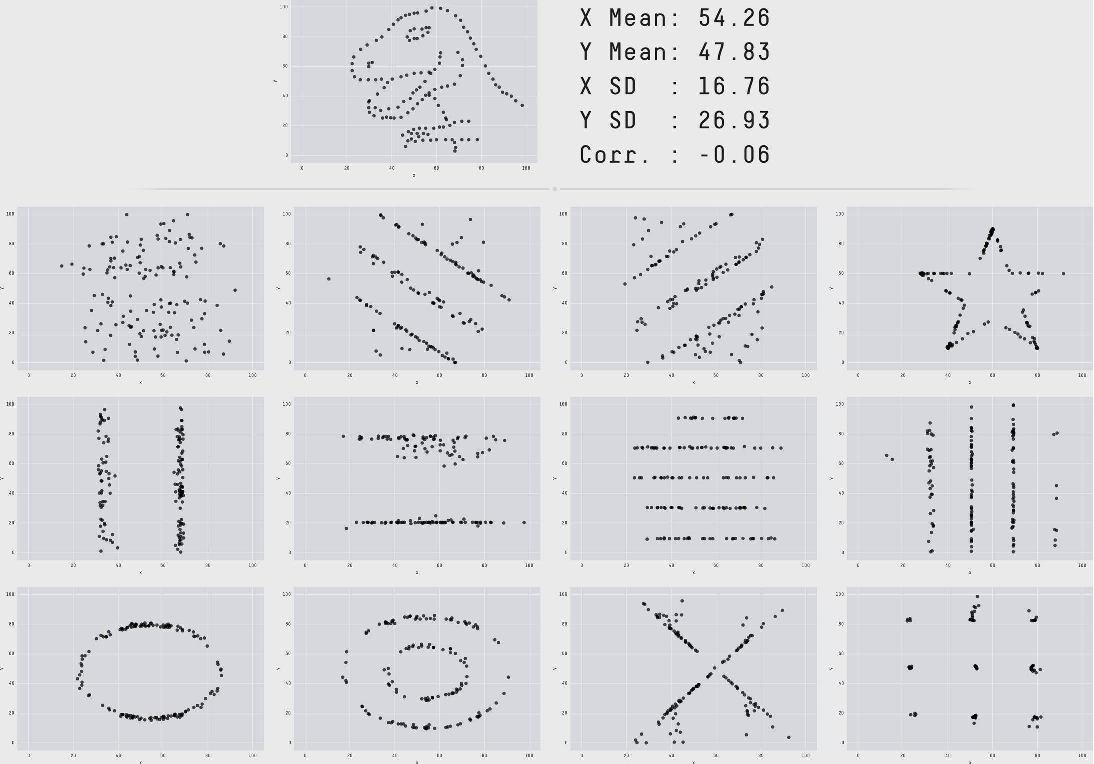
\includegraphics[width=0.92\linewidth]{figures/datasaurus_dozen.pdf}
\caption{The Datasaurus Dozen (Matejka \& Fitzmaurice, 2017)~\cite{matejka2017same}. All 13 distinct bivariate distributions share identical summary statistics up to two decimal places: horizontal mean $\bar{x} = 54.26$, vertical mean $\bar{y} = 47.83$, standard deviations $s_x = 16.76, s_y = 26.93$, and Pearson correlation coefficient $r = -0.06$. Yet their true empirical geometries range from a Tyrannosaurus Rex to concentric rings, starbursts, and parallel lines.}
\label{fig:slide_datasaurus}
\end{figure}

Figure~\ref{fig:slide_datasaurus} illustrates the \textbf{Datasaurus Dozen} experiment~\cite{matejka2017same}, an eloquent modern generalization of Anscombe's 1973 quartet. Each of the 13 bivariate datasets consists of 142 points and exhibits identical numerical properties to two decimal places:
\begin{equation}
\bar{x} = 54.26, \quad \bar{y} = 47.83, \quad s_x = 16.76, \quad s_y = 26.93, \quad r_{xy} = -0.06.
\label{eq:datasaurus_stats}
\end{equation}
An algorithm or practitioner relying solely on these metrics would conclude that all 13 datasets represent identical physical mechanisms. Yet inspecting the geometric plots reveals entirely distinct realities: one is a dinosaur, another is a high-density cluster surrounded by an outer ring, and another is a sequence of discrete vertical stripes.

To understand mathematically why summary statistics fail so catastrophically, consider the analytical formula for the \textbf{sample Pearson correlation coefficient} $r_{xy}$:
\begin{equation}
r_{xy} = \frac{\sum_{i=1}^N (x_i - \bar{x})(y_i - \bar{y})}{\sqrt{\sum_{i=1}^N (x_i - \bar{x})^2} \sqrt{\sum_{i=1}^N (y_i - \bar{y})^2}}.
\label{eq:pearson_correlation_formula}
\end{equation}
Equation~\eqref{eq:pearson_correlation_formula} measures exclusively \textbf{first-order linear co-variation}. When the underlying structural relationship is non-linear (such as a circle $x^2 + y^2 = R^2$, a parabola $y = x^2$, or a complex contour), deviations above and below the mean cancel out symmetrically in the numerator $\sum (x_i - \bar{x})(y_i - \bar{y}) \approx 0$. 

Furthermore, summary statistics completely discard:
\begin{itemize}[noitemsep]
  \item High-order statistical moments: skewness ($\mathbb{E}[(X-\mu)^3]/\sigma^3$) and kurtosis ($\mathbb{E}[(X-\mu)^4]/\sigma^4$).
  \item Multi-modal cluster topology and manifold connectivity.
  \item Heavy-tailed extreme values and catastrophic outlier distributions.
\end{itemize}
Hence, the golden imperative of machine learning: \textbf{Never trust summary statistics alone; always visualize and deeply inspect the data before modeling.}

\subsection{Pillar 1: Observe the data (Exploratory visualization and feature spaces)}
\label{sec:pillar_1_observe}

The first rule of machine learning is to open the dataset directory and directly examine the individual instances. In tabular domains or low-dimensional problems ($d \le 3$), scatter plots, histograms, and pair-wise correlation grids allow immediate visual diagnosis.

However, modern deep learning typically operates on extremely high-dimensional spaces: an uncompressed $256 \times 256$ RGB image lives in $\mathbb{R}^{196,608}$, and feature embeddings extracted from foundation models live in $\mathbb{R}^{1,024}$ or $\mathbb{R}^{4,096}$. Humans cannot directly visualize geometries beyond three dimensions. To observe such data, practitioners deploy mathematical projection and dimensionality reduction techniques:
\begin{itemize}[noitemsep]
  \item \textbf{Principal Component Analysis (PCA)}: Identifies the orthogonal directions of maximal variance by computing the eigenvectors of the empirical covariance matrix $\mathbf{\Sigma} = \frac{1}{N}\mathbf{X}^\top \mathbf{X}$, projecting $d$-dimensional representations onto the leading 2D or 3D principal sub-space.
  \item \textbf{Non-linear Manifold Learning}: Methods such as $t$-Distributed Stochastic Neighbor Embedding ($t$-SNE) and Uniform Manifold Approximation and Projection (UMAP) preserve local neighborhood topologies, unrolling complex non-linear manifolds into interpretable 2D diagnostic visual maps.
\end{itemize}

\paragraph{Critical oral exam insight: Knowing your dataset.}
In the oral examination, a fundamental line of questioning focuses on dataset mastery: \emph{Which benchmark did you use in your project or paper analysis? What semantic object categories does it contain? How many total instances are present, and what is the exact sample distribution across classes?} A candidate who views data as an interchangeable numeric matrix without knowing its class taxonomy, sensor resolution, or subgroup composition demonstrates a shallow understanding. A true machine learner understands the physical reality generating each feature coordinate.

\subsection{Pillar 2: Summarize uncertainty (Distributions and probabilistic frameworks)}
\label{sec:pillar_2_uncertainty}

Rather than condensing a feature coordinate into a single scalar average $\bar{x}$, rigorous data analysis models uncertainty through full probability distributions:
\begin{equation}
p(\mathbf{x}) \quad \text{or} \quad p(\mathbf{x} \mid y).
\end{equation}
As derived in Section~\ref{sec:data_uncertainty}, uncertainty comprises both irreducible sensor stochasticity (aleatoric) and epistemic parameter ignorance arising from data sparsity. In safety-critical applications—such as autonomous navigation or medical oncology—a point prediction $\hat{y} = f(\mathbf{x})$ without an accompanying confidence interval or posterior distribution $p(y \mid \mathbf{x})$ is dangerous. Modeling the full distribution provides the foundational calculus for Bayes decision theory, hypothesis testing, and risk-aware decision boundaries.

\subsection{Pillar 3: Search for constraints and invariances (Prior knowledge)}
\label{sec:pillar_3_prior_knowledge}

Without prior knowledge, an algorithm facing a finite dataset $\mathcal{D}_N$ must search through the uncountably infinite universe of mathematical functions that interpolate the points. Prior domain knowledge acts as a powerful mathematical filter, restricting the hypothesis space $\mathcal{H}$ to functions that obey known physical laws, geometric symmetries, and environmental constraints.

\paragraph{Historical case study: Alan Turing and the Enigma machine.}
The power of prior constraints to collapse search complexity is historically illustrated by Alan Turing's codebreaking triumph at Bletchley Park during World War II (dramatized in \emph{The Imitation Game}). The German military Enigma cipher machine possessed an astronomical keyspace: with multiple rotating rotors, ring settings, and a plugboard (\emph{Steckerbrett}), the machine offered approximately $1.5 \times 10^{20}$ possible daily wiring configurations. A brute-force search over this space was physically impossible, even with electromechanical computing machines (the \emph{Bombes}), within the daily 24-hour window before settings changed.

Turing's decisive insight was discovering an empirical invariance—a deterministic constraint in the communication protocol. German telegraph operators routinely began their first daily transmissions at exactly 06:00 with standardized meteorological reports containing invariant phrasing:
\begin{equation}
\text{\emph{Wetterbericht}} \quad (\text{"Weather Report"}),
\end{equation}
and frequently concluded messages with the obligatory military salutation:
\begin{equation}
\text{\emph{Heil Hitler}}.
\end{equation}
These predictable, recurring plaintext sequences (known as \textbf{cribs}) provided deterministic anchors between known plaintext and observed ciphertext. By enforcing these known linguistic constraints, Turing's Bombe did not have to search the entire combinatorial space of billions of permutations; the search space collapsed to a tiny feasible subset that the machines could eliminate in minutes.

\paragraph{Machine learning formulation.}
In statistical machine learning, prior knowledge functions in precisely the same manner: it dramatically reduces the volume of the hypothesis space $|\mathcal{H}|$ that must be searched during optimization. 
\begin{itemize}[noitemsep]
  \item If domain physics indicates that a signal originates from a continuous periodic industrial process (e.g., turbine vibration or seasonal temperature oscillation), searching over arbitrary high-degree polynomials is wasteful and leads to catastrophic boundary oscillations. Instead, the practitioner restricts $\mathcal{H}$ to a sinusoidal basis family:
  \begin{equation}
  f(x; \mathbf{w}) = A \sin(\omega x + \phi) + b.
  \end{equation}
  \item In computer vision, our prior knowledge that physical objects retain their semantic identity regardless of where they appear in the visual field directly justifies imposing \textbf{translation equivariance} via Convolutional Neural Networks ($f(T_g(\mathbf{x})) = T_g(f(\mathbf{x}))$), eliminating billions of redundant parameters compared to unconstrained fully connected layers.
\end{itemize}
Prior knowledge is the most effective regularizer: it saves optimization time, prevents overfitting, and minimizes the sample complexity required to achieve high generalization.

\subsection{Pillar 4: Find a model to explain the data (Families, capacity, and coordinate linearization)}
\label{sec:pillar_4_model_family}

Once data has been observed and prior constraints identified, the machine learner selects an appropriate mathematical model family $f(\mathbf{x}; \boldsymbol{\theta})$ to explain the relationship between input $\mathbf{x}$ and target $y$.

\paragraph{Model family complexity trade-offs.}
Consider fitting a two-dimensional dataset $\{(x_i, y_i)\}_{i=1}^N$:
\begin{itemize}[noitemsep]
  \item \textbf{Degree 1 Polynomial (Linear)}: $y = w_1 x + w_0$. Imposes high inductive bias; requires fitting only 2 scalar parameters. Fast to optimize, but suffers from underfitting if the true physical relationship exhibits curvature.
  \item \textbf{Degree 2 Polynomial (Quadratic)}: $y = w_2 x^2 + w_1 x + w_0$. Requires fitting 3 parameters; models parabolic trajectories.
  \item \textbf{Degree 3 Polynomial (Cubic)}: $y = w_3 x^3 + w_2 x^2 + w_1 x + w_0$. Requires fitting 4 parameters; captures inflection points.
  \item \textbf{Parametric 2D Curves}: Expressing coordinates parametrically as $(x(t), y(t)) = (a_x t + b_x, a_y t + b_y)$ introduces 4 parameters. While more flexible for trajectories, it doubles optimization requirements relative to a standard Cartesian linear model.
\end{itemize}

\paragraph{Coordinate transformations and the power of linearization.}
An expert machine learner does not merely increase model capacity when faced with geometrically complex data; they look for coordinate transformations that simplify the problem.

Consider a dataset whose points form an Archimedean spiral or circular ring centered at $(x_c, y_c)$. In standard Cartesian coordinates $(x, y)$, describing this trajectory with an explicit algebraic function $y = f(x)$ is impossible because the curve fails the vertical line test (a single $x$ maps to multiple values of $y$). Attempting to fit a high-degree Cartesian polynomial results in severe optimization instabilities.

Instead of adopting an unwieldy high-capacity black box, the practitioner shifts the origin to the empirical data centroid $(x_c, y_c)$ and transforms the coordinates into polar space:
\begin{equation}
r = \sqrt{(x - x_c)^2 + (y - y_c)^2}, \quad \theta = \operatorname{atan2}(y - y_c, x - x_c).
\label{eq:polar_transformation}
\end{equation}
In polar coordinates $(r, \theta)$, the complex spiral trajectory unrolls into an elementary linear relationship:
\begin{equation}
r(\theta) = a \theta.
\label{eq:linear_polar_spiral}
\end{equation}
By simply changing the geometric frame of reference, the learning problem reduces from fitting an intractable non-linear model to fitting a \textbf{single linear parameter} $a$! Mathematical sophistication in representation simplifies computational optimization.

\subsection{Pillar 5: Represent the data (Handcrafted features vs. geometric dimensionality)}
\label{sec:pillar_5_representation}

Learning algorithms do not ingest raw physical reality; they process mathematical representations. In classical machine learning (from the 1980s through 2010), representations were constructed via manual feature engineering guided by human domain experts.

\paragraph{The Fisher Iris paradigm.}
Consider the classical problem of classifying botanical species of Iris flowers into \emph{Iris setosa} and \emph{Iris versicolor}. Feeding raw, unprocessed botanical descriptions to a classifier yields poor results. Instead, a human botanical expert identifies the two morphological measurements that carry discriminative power:
\begin{equation}
x_1 = \text{Petal Length}, \quad x_2 = \text{Sepal Length}.
\end{equation}
Projecting each flower instance into this engineered 2D feature space $\mathbf{x} = [x_1, x_2]^\top \in \mathbb{R}^2$ separates the two species cleanly, allowing a simple Support Vector Machine (SVM) or linear hyperplane to achieve near-perfect classification.

\paragraph{Resolving non-separable distributions: Two foundational strategies.}
When classes overlap in a chosen feature space and cannot be separated linearly, the machine learner faces two distinct design choices:
\begin{enumerate}
  \item \textbf{Invest in Classifier Complexity}: Retain the current low-dimensional feature space, but replace the linear classifier with an intricate, highly non-linear decision boundary (e.g., high-degree polynomial kernels, deep decision trees, or multi-layer neural networks).
  \item \textbf{Invest in Representation (Lifting the Dimension)}: Consult domain experts or extract additional feature measurements (e.g., adding $x_3 = \text{Petal Width}$ and $x_4 = \text{Sepal Width}$). By embedding the data into a higher-dimensional space $\mathbb{R}^d$ ($d > 2$), entangled clusters disentangle naturally, allowing an elementary linear classifier to separate them with high margin.
\end{enumerate}

\paragraph{Dimensionality reduction and manifold unrolling.}
Conversely, when raw data is unnecessarily high-dimensional (e.g., 100 sensor readings that are heavily correlated), the data may lie on a low-dimensional intrinsic manifold (e.g., a 2D sheet embedded in $\mathbb{R}^3$). In such cases, applying linear PCA or non-linear manifold unrolling reduces dimensionality, eliminates multicollinearity, suppresses measurement noise, and circumvents the curse of dimensionality.

\subsection{Pillar 6: Joint end-to-end learning via computing power (The playing cards analogy)}
\label{sec:pillar_6_joint_learning}

The decisive paradigm shift of the 2010 Deep Learning revolution was abandoning decoupled manual feature engineering in favor of \textbf{end-to-end joint representation learning}.

\begin{figure}[htbp]
\centering
\begin{tikzpicture}[>=Stealth, node distance=1.2cm, scale=0.95, every node/.style={transform shape}]
  % Styles
  \tikzset{
    card/.style = {draw=politoNavy, fill=white, rounded corners=4pt, minimum width=1.2cm, minimum height=1.65cm, line width=1.1pt, font=\bfseries},
    taskbox/.style = {draw=deepdiveTeal, fill=white, rounded corners=5pt, line width=1.1pt, inner sep=6pt, font=\small, align=left}
  }

  % Raw Playing Cards Deck
  \node[font=\bfseries\normalsize, text=politoNavy] (title) at (0, 3.2) {Raw Observation: Standard 52-Card Deck $\mathbf{x} \in \mathcal{X}$};

  % Visual Cards
  \node[card] (c1) at (-2.2, 1.8) {$\spadesuit$\,\text{Q}};
  \node[card, draw=examred, text=examred] (c2) at (-0.75, 1.8) {$\heartsuit$\,\text{A}};
  \node[card] (c3) at (0.75, 1.8) {$\clubsuit$\,\text{K}};
  \node[card, draw=examred, text=examred] (c4) at (2.2, 1.8) {$\diamondsuit$\,10};

  % Intrinsic Features Panel
  \node[draw=gray!60, fill=gray!8, rounded corners=4pt, inner sep=5pt, font=\scriptsize, align=center] (feat) at (0, 0.4) {
    \textbf{Generic Intrinsic Attributes:}\\
    $\text{Rank} \in \{\text{A}, 2, \dots, \text{K}\}, \quad \text{Suit} \in \{\spadesuit, \heartsuit, \clubsuit, \diamondsuit\}, \quad \text{Color} \in \{\text{Black}, \text{Red}\}$
  };

  % Downstream Task Nodes
  \node[taskbox, draw=politoNavy] (t1) at (-4.2, -1.8) {
    \textbf{Task 1: Poker}\\
    \rule{3.2cm}{0.4pt}\\
    $\bullet$ \textbf{Rank}: Crucial (straights, pairs)\\
    $\bullet$ \textbf{Suit}: Crucial (flushes)\\
    $\bullet$ \textbf{Color}: \textit{Redundant / Irrelevant}
  };

  \node[taskbox, draw=intuitiongreen] (t2) at (0, -1.8) {
    \textbf{Task 2: Blackjack}\\
    \rule{3.2cm}{0.4pt}\\
    $\bullet$ \textbf{Rank}: Additive value only\\
    $\bullet$ \textbf{Suit}: \textit{Completely irrelevant}\\
    $\bullet$ \textbf{Color}: \textit{Completely irrelevant}
  };

  \node[taskbox, draw=examred] (t3) at (4.2, -1.8) {
    \textbf{Task 3: Hearts}\\
    \rule{3.2cm}{0.4pt}\\
    $\bullet$ \textbf{Rank \& Suit Jointly}:\\
    \quad $\spadesuit\,\text{Q} \implies -13$ penalty pts!\\
    \quad $\heartsuit \implies -1$ pt each\\
    $\bullet$ \textbf{Color}: \textit{No independent role}
  };

  % Connecting Arrows
  \draw[->, very thick, politoNavy] (feat.south) -- ++(0, -0.3) -| (t1.north) 
    node[pos=0.25, above, font=\scriptsize\bfseries, text=politoNavy] {Task Mapping $\phi_{\text{poker}}(\mathbf{x})$};
  \draw[->, very thick, intuitiongreen] (feat.south) -- (t2.north)
    node[pos=0.45, right, font=\scriptsize\bfseries, text=intuitiongreen] {$\phi_{\text{blackjack}}(\mathbf{x})$};
  \draw[->, very thick, examred] (feat.south) -- ++(0, -0.3) -| (t3.north)
    node[pos=0.25, above, font=\scriptsize\bfseries, text=examred] {$\phi_{\text{hearts}}(\mathbf{x})$};

  % Core Moral Callout
  \node[draw=politoNavy, fill=politoNavy!5, rounded corners=5pt, line width=1.2pt, font=\small, align=center, inner sep=6pt] at (0, -3.8) {
    \textbf{The Representation Principle:} There is no such thing as an optimal ``universal'' feature set in a vacuum.\\
    Feature utility $\phi(\mathbf{x})$ is \textbf{strictly conditioned} on the target task $\mathcal{T}$ and objective loss $\mathcal{L}(\hat{y}, y)$.
  };
\end{tikzpicture}
\caption{The playing card representation analogy: context-dependent, task-driven features. In a standard 52-card deck, cards possess invariant intrinsic properties (rank, suit, and color). However, the utility of these features depends entirely on the game being played: in Hearts, the Queen of Spades carries devastating negative penalty points; in Poker, flushes require tracking suits while rank determines straights; in Blackjack, suits and colors are completely irrelevant and only numeric card values matter.}
\label{fig:slide_card_representation}
\end{figure}

\paragraph{The playing cards analogy: Features are strictly task-driven.}
Why must representation learning be coupled directly to the learning task? The answer is illustrated by the card-game analogy depicted in Figure~\ref{fig:slide_card_representation}. 

A standard deck of playing cards contains 52 elements, each possessing fixed intrinsic attributes:
\begin{equation}
\text{Rank} \in \{\text{Ace}, 2, \dots, \text{King}\}, \quad \text{Suit} \in \{\heartsuit, \diamondsuit, \clubsuit, \spadesuit\}, \quad \text{Color} \in \{\text{Red}, \text{Black}\}.
\end{equation}
If you ask an expert to build a "universal feature representation" for a playing card, they cannot answer without knowing the game to be played:
\begin{itemize}[noitemsep]
  \item In \textbf{Poker}, suit is vital for detecting flushes, and rank order is vital for straights, whereas color is redundant.
  \item In \textbf{Blackjack}, suit and color are completely irrelevant; only the additive numeric value of the rank matters.
  \item In \textbf{Hearts}, the Queen of Spades ($\text{Q}\spadesuit$) carries a severe 13-point penalty, making that specific combination of suit and rank uniquely critical, while diamond cards carry zero penalty.
\end{itemize}
This pedagogical example reveals a core axiom of modern machine learning: \textbf{There is no universally optimal feature representation; features only make sense relative to the specific task $\mathcal{T}$ being solved!}

\paragraph{Shallow vs. Deep learning architectures.}
This principle explains why shallow machine learning frequently hit performance ceilings:
\begin{equation}
\text{Raw Data } \mathbf{x} \xrightarrow[\text{Human Expert}]{\text{Fixed Handcrafted Features}} \boldsymbol{\phi}(\mathbf{x}) \xrightarrow[\text{Learned}]{\text{Shallow Model}} \hat{y}.
\end{equation}
In shallow ML, the feature extractor $\boldsymbol{\phi}(\mathbf{x})$ is fixed and decoupled from the classifier. If the human expert's handcrafted descriptors omit subtle correlations essential for the downstream task, the classifier can never recover them.

In contrast, Deep Learning unifies representation extraction and task optimization into a single differentiable pipeline:
\begin{equation}
\text{Raw Data } \mathbf{x} \xrightarrow[\text{Differentiable Layers}]{\mathbf{W}_1, \mathbf{W}_2, \dots, \mathbf{W}_{L-1}} \mathbf{h}_{L-1}(\mathbf{x}) \xrightarrow[\text{Classification Head}]{\mathbf{W}_L} \hat{y}.
\end{equation}
Driven by the backpropagation of the task-specific loss gradient $\nabla_{\mathbf{W}} \ell(\hat{y}, y)$, the internal layers dynamically mold their intermediate representations $\mathbf{h}_l$ specifically to solve task $\mathcal{T}$.

\paragraph{ImageNet and hierarchical feature emergence.}
In the seminal 2012 AlexNet architecture trained on the 1,000-class ImageNet benchmark, inspecting the learned convolutional filter weights revealed a structured hierarchy of representation:
\begin{itemize}[noitemsep]
  \item \textbf{Early Layers (Layers 1--2)}: Extract generic low-level visual primitives: oriented Gabor-like edge filters across multiple angles, spatial frequency bars, and localized color blobs.
  \item \textbf{Intermediate Layers (Layers 3--4)}: Group low-level edges into composite textures, corners, repetitive grids, and structural object parts (e.g., circular wheel rims, mesh grilles, and animal eyes).
  \item \textbf{Deep Layers (Layer 5 and fully connected heads)}: Assemble object parts into holistic class-specific semantic representations (e.g., complete dog faces, bird beaks, and bicycle frames).
\end{itemize}
This hierarchical decomposition was not programmed by humans; it emerged autonomously from raw pixels driven entirely by gradient optimization on the cross-entropy task loss.

\subsection{Pillar 7: Avoid data bias, spurious correlations, and enforce fairness}
\label{sec:pillar_7_avoid_bias}

The final pillar governs the ethical and epistemological reliability of deployed models. A pervasive myth in society is that mathematical algorithms are inherently objective and immune to human prejudice. 

In reality, \textbf{machine learning models are objective only in the sense that they faithfully optimize their loss function on whatever empirical data they are fed.} If the training data contains historical societal inequities, unrepresentative demographic sampling, or spurious statistical artifacts, the model will not correct them; it will exploit them as optimal predictive shortcuts.

---

\section{Societal consequences of bias and the algorithmic frontier}
\label{sec:societal_bias_and_fairness}

When machine learning systems are deployed in real-world institutions—such as criminal justice, credit scoring, medical triage, and hiring—data bias ceases to be a theoretical optimization nuisance and becomes an active source of systemic harm.

\subsection{Spurious correlations as algorithmic shortcuts: The doctor vs. nurse dilemma}
\label{sec:spurious_shortcuts}

Machine learning models optimize purely for accuracy under their training distribution. When presented with training datasets that reflect historical gender imbalances in professional occupations, computer vision models learn to rely on spurious demographic shortcuts rather than true semantic features.

In benchmark experiments on occupation classification from photographs:
\begin{itemize}[noitemsep]
  \item A human expect the classifier to distinguish a doctor from a nurse by examining functional attire: stethoscopes, surgical masks, white laboratory coats, or specialized instruments.
  \item Instead, feature attribution maps (such as Grad-CAM) revealed that the deep networks were focusing directly on the subject's face to classify \textbf{gender}: if the subject was male, the network predicted "Doctor"; if the subject was female, it predicted "Nurse".
\end{itemize}
Because the scraped web training data had a high proportion of male doctors and female nurses, the model discovered that facial gender recognition was an easy statistical shortcut to achieve high training accuracy with minimal gradient effort. 

When deployed in clinical environments where female doctors and male nurses are present, the model failed catastrophically. This failure illustrates the fundamental machine learning adage: \textbf{"Garbage in, garbage out"}—if an algorithm is trained on biased data, it produces biased, untrustworthy predictions.

\subsection{The COMPAS recidivism case study and mathematical fairness}
\label{sec:compas_case_study}

The most consequential and widely analyzed real-world failure of algorithmic decision-making occurred in the United States criminal justice system with the \textbf{COMPAS} (Correctional Offender Management Profiling for Alternative Sanctions) algorithm, developed by Northpointe (now Equivant)~\cite{angwin2016machine}.

\paragraph{Algorithmic deployment in pretrial detention.}
COMPAS is a commercial risk-assessment instrument used by judges in multiple US jurisdictions to predict a criminal defendant's likelihood of reoffending (recidivism) within two years. The algorithm outputs a decile risk score from 1 (lowest risk) to 10 (highest risk). Judges routinely consult this scalar score when deciding whether a defendant should be granted pretrial release on bail or remanded to prison pending trial.

COMPAS was trained on historical criminal records and arrest histories spanning decades—a historical record heavily shaped by racially disparate policing practices, stop-and-frisk policies, and socio-economic profiling.

\paragraph{The 2016 ProPublica investigative audit.}
In a landmark 2016 investigative analysis, journalists Julia Angwin, Jeff Larson, Surya Mattu, and Lauren Kirchner from \emph{ProPublica} audited the COMPAS risk scores and subsequent two-year arrest records of over 7,000 individuals arrested in Broward County, Florida~\cite{angwin2016machine}. 

While the algorithm did not explicitly receive race as an input feature coordinate, it took 137 questionnaire responses and historical arrest counts that served as close proxies for socio-economic background and race. When ProPublica evaluated the accuracy of COMPAS across demographic groups, they discovered a severe, systematic racial asymmetry in prediction errors:
\begin{itemize}
  \item \textbf{Disparate False Positive Rate (FPR)}: Among defendants who \textbf{did not reoffend} during the subsequent two-year follow-up window, Black defendants were mistakenly classified as medium or high risk at almost \textbf{twice the rate} of White non-reoffenders:
  \begin{equation}
  \text{FPR}_{\text{Black}} = 44.9\% \quad \text{vs.} \quad \text{FPR}_{\text{White}} = 23.5\%.
  \label{eq:compas_fpr}
  \end{equation}
  \item \textbf{Disparate False Negative Rate (FNR)}: Conversely, among defendants who \textbf{did reoffend} within two years, White defendants were mistakenly classified as low risk at almost \textbf{twice the rate} of Black reoffenders:
  \begin{equation}
  \text{FNR}_{\text{White}} = 47.7\% \quad \text{vs.} \quad \text{FNR}_{\text{Black}} = 28.0\%.
  \label{eq:compas_fnr}
  \end{equation}
\end{itemize}
In human terms, the algorithm exhibited a severe asymmetric bias: it systematically projected future criminality onto innocent Black individuals while extending undue leniency and benefit of the doubt to White individuals who subsequently committed crimes.

\paragraph{The Impossibility Theorem of Algorithmic Fairness.}
The COMPAS controversy sparked an intense mathematical debate between Northpointe and academic computer scientists. Northpointe defended the tool by proving that COMPAS satisfied \textbf{Predictive Parity (Calibration within Groups)}: for any given risk score $s$ (e.g., score $= 7$), the probability that a defendant reoffends is roughly equal regardless of race:
\begin{equation}
P(Y = 1 \mid S = s, A = \text{Black}) \approx P(Y = 1 \mid S = s, A = \text{White}).
\label{eq:predictive_parity}
\end{equation}
ProPublica, by contrast, evaluated the algorithm according to \textbf{Error Rate Parity (Equalized Odds / Separation)}: requiring equal false positive rates and false negative rates across groups:
\begin{equation}
P(\hat{Y} = 1 \mid Y = 0, A = \text{Black}) \stackrel{?}{=} P(\hat{Y} = 1 \mid Y = 0, A = \text{White}).
\label{eq:error_rate_parity}
\end{equation}

In 2016, computer scientists Jon Kleinberg, Sendhil Mullainathan, and Manish Raghavan~\cite{kleinberg2016inherent} (and independently Alexandra Chouldechova) proved a foundational mathematical theorem known as the \textbf{Impossibility Theorem of Fairness}:

\begin{theorem}[Fairness Impossibility Theorem~\cite{kleinberg2016inherent}]
Let $Y \in \{0, 1\}$ be the true binary outcome, $\hat{Y} \in \{0, 1\}$ be the binary decision, and $A \in \{a, b\}$ be a sensitive demographic attribute. Suppose the base rates of the two groups are unequal:
\begin{equation}
P(Y = 1 \mid A = a) \ne P(Y = 1 \mid A = b),
\end{equation}
and the classifier is not a perfect predictor (i.e., its error rate is non-zero). Then, it is \textbf{mathematically impossible} for any algorithm to simultaneously satisfy:
\begin{enumerate}[noitemsep]
  \item \textbf{Calibration (Predictive Parity)}: $P(Y = 1 \mid \hat{Y} = 1, A = a) = P(Y = 1 \mid \hat{Y} = 1, A = b)$.
  \item \textbf{Equal False Positive Rates}: $P(\hat{Y} = 1 \mid Y = 0, A = a) = P(\hat{Y} = 1 \mid Y = 0, A = b)$.
  \item \textbf{Equal False Negative Rates}: $P(\hat{Y} = 0 \mid Y = 1, A = a) = P(\hat{Y} = 0 \mid Y = 1, A = b)$.
\end{enumerate}
\end{theorem}
Because historical arrest base rates differed between demographic groups due to structural socio-economic inequalities, satisfying calibration mathematically forced COMPAS to produce asymmetric false positive rates! 

This mathematical reality underscores why algorithmic fairness cannot be resolved purely by code: practitioners must consciously choose which fairness definition to prioritize based on legal, ethical, and societal values.

\subsection{Legal and regulatory safeguards: The EU AI Act (August 2024)}
\label{sec:eu_ai_act}

In response to scandals such as COMPAS and predatory biometric profiling, governments have instituted binding legal regulations. In \textbf{August 2024}, the European Union enacted into law the \textbf{Artificial Intelligence Act (EU AI Act)}, establishing the world's first comprehensive horizontal legal framework for AI governance.

The EU AI Act establishes a four-tiered risk-based regulatory pyramid:
\begin{enumerate}
  \item \textbf{Unacceptable Risk (Prohibited)}: AI systems that pose an intolerable threat to human safety and fundamental rights are banned outright. This includes government social credit scoring, cognitive behavioral manipulation targeting vulnerable populations, biometric categorization based on political/philosophical beliefs, and real-time biometric identification in public spaces by law enforcement (with narrow judicial exceptions).
  \item \textbf{High-Risk (Strictly Regulated)}: Systems deployed in critical sectors that directly impact human livelihoods, health, safety, and civil rights. Crucially, the EU AI Act classifies AI used in \textbf{the administration of justice, law enforcement, judicial bail decisions, credit scoring, employment recruitment, education grading, and critical infrastructure} as \textbf{High-Risk}.
  \item \textbf{General Purpose AI (GPAI)}: Large foundation models (e.g., frontier LLMs) must comply with transparency mandates, copyright documentation, and systemic risk assessments for frontier capabilities exceeding $10^{25}$ FLOPs.
  \item \textbf{Minimal / Low Risk}: Systems like spam filters, AI recommendation engines, or video games, which remain largely unconstrained.
\end{enumerate}

\paragraph{Mandatory compliance for High-Risk AI.}
Under the EU AI Act, systems operating in the justice and law enforcement domains (such as COMPAS-like recidivism tools) face stringent legal obligations before they can enter the EU market:
\begin{itemize}[noitemsep]
  \item \textbf{Mandatory Data Governance}: Training, validation, and testing datasets must be vetted for representative demographic balance, data quality, and statistical bias mitigation prior to training.
  \item \textbf{Mandatory Human Oversight}: AI models cannot automate judicial sentences or legal determinations autonomously. A qualified human magistrate must retain effective supervisory control (\emph{human-in-the-loop}), with full authority to override, reject, or ignore algorithmic outputs.
  \item \textbf{Traceability and Audit Logs}: High-risk systems must automatically log their operating states, input distributions, and decision paths to facilitate post-hoc judicial audits.
\end{itemize}
While the EU AI Act legally applies only within European jurisdiction, its extraterritorial scope binds any international entity or US provider deploying AI systems whose outputs affect individuals residing within the European Union.

\subsection{Domain shift, Sim-to-Real gap, and the limits of i.i.d. generalization}
\label{sec:domain_shift_and_sim2real}

Statistical learning theory rests entirely on the foundational assumption that training samples and future deployment test samples are drawn \textbf{independently and identically distributed (i.i.d.)} from the exact same stationary probability distribution:
\begin{equation}
p_{\text{train}}(\mathbf{x}, y) \equiv p_{\text{test}}(\mathbf{x}, y) = p_{\text{data}}(\mathbf{x}, y).
\label{eq:iid_stationarity_assumption}
\end{equation}
In real-world deployment, this assumption is universally violated.

\begin{figure}[htbp]
\centering
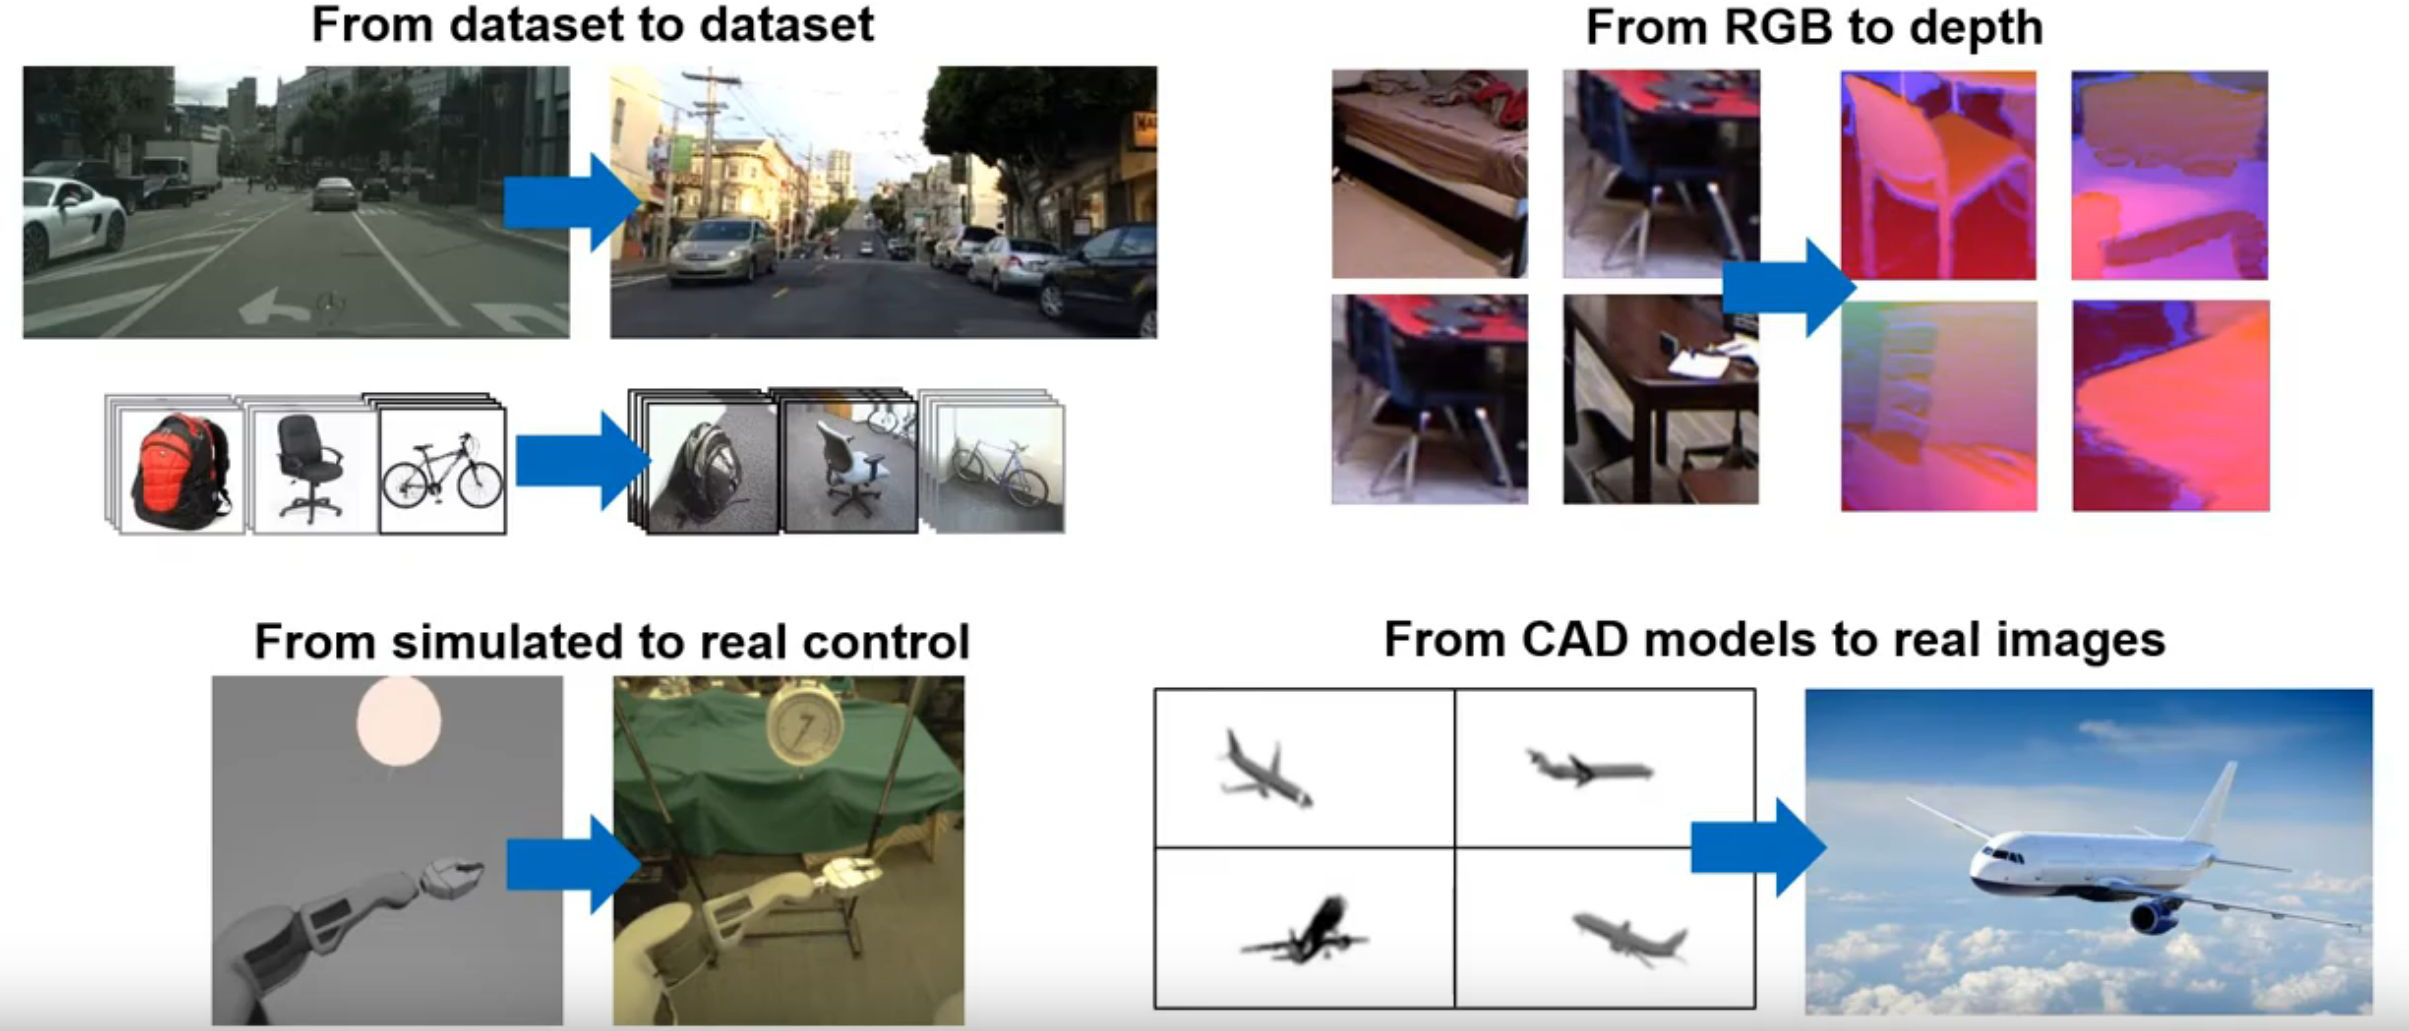
\includegraphics[width=0.92\linewidth]{figures/domain_shift_office31.png}
\caption{Dataset bias and domain shift (Torralba \& Efros, 2011; Saenko et al., 2010)~\cite{torralba2011unbiased,saenko2010adapting}. When an image classifier trained on high-quality product images (e.g., Amazon catalogue photos) is deployed on real-world webcam photos or mobile phone snapshots, accuracy drops precipitously due to distribution shift across lighting, background clutter, and camera angles.}
\label{fig:slide_dataset_bias}
\end{figure}

As shown in Figure~\ref{fig:slide_dataset_bias}, when models encounter \textbf{domain shift}, test accuracy drops precipitously. The two primary mathematical forms of domain shift are:
\begin{itemize}
  \item \textbf{Covariate Shift}: The marginal input feature distribution shifts ($p_{\text{train}}(\mathbf{x}) \ne p_{\text{test}}(\mathbf{x})$), while the posterior conditional label boundary remains invariant ($P(y \mid \mathbf{x})$ is constant).
  \item \textbf{Concept Drift}: The conditional label distribution itself changes ($P_{\text{train}}(y \mid \mathbf{x}) \ne P_{\text{test}}(y \mid \mathbf{x})$), meaning identical input observations map to different semantic classes over time.
\end{itemize}

\paragraph{Autonomous driving and the Sim-to-Real gap.}
A vivid empirical example occurs in autonomous robotics and self-driving vehicles:
\begin{itemize}
  \item \textbf{Geographic and Environmental Domain Shift}: An autonomous driving perception network trained exclusively on camera footage collected in sunny daylight conditions in Rome will fail catastrophically when deployed during a heavy snowstorm at night in Beijing. Lighting conditions, road textures, precipitation scatter, and pedestrian behaviors change drastically ($p_{\text{train}}(\mathbf{x}) \ne p_{\text{test}}(\mathbf{x})$).
  \item \textbf{The Sim-to-Real Gap}: Autonomous robots cannot be trained from scratch in physical reality because random exploration would cause physical collisions, vehicle crashes, and immense financial cost. Consequently, roboticists and autonomous vehicle developers train perception systems inside high-fidelity 3D synthetic simulators or game engines like \textbf{Grand Theft Auto V (GTA V)} and CARLA. 
\end{itemize}
While synthetic video game data is infinitely cheap, fully scalable, and comes with free, perfect pixel-level semantic segmentation annotations, real-world deployment reveals a severe \textbf{Sim-to-Real domain gap}. Synthetic graphics rendering engines lack the high-frequency physical noise, optical aberrations, dynamic specular reflections, and chaotic imperfections of the physical world. A model that achieves $99\%$ semantic segmentation accuracy inside GTA V drops precipitously when tested on physical highway cameras.

Overcoming this gap requires modern techniques beyond classical i.i.d. learning:
\begin{itemize}[noitemsep]
  \item \textbf{Unsupervised Domain Adaptation (UDA)}: Aligning source and target feature representations via adversarial minimax objectives (e.g., Domain-Adversarial Neural Networks, DANN~\cite{ganin2016domain}).
  \item \textbf{Domain Randomization}: Randomizing simulation lighting, camera angles, textures, and weather dynamics during synthetic training so that physical reality appears to the network as merely another synthetic variation.
  \item \textbf{Continual / Lifelong Learning}: Updating network parameters online in response to non-stationary environments without catastrophically forgetting previously mastered domains.
\end{itemize}
The study of dataset bias, domain adaptation, and statistical robustness represents the true frontier of modern machine learning, bridging laboratory benchmarks to robust physical reality.

